%%%%%%%%%%%%%%%%%%%%%%%%%%%%%%%%%%%%%%%%%%%%%%%%%%%%%%%%%%%%%%%%%
\chapter{SIMULATIONS AND RESULTS}\label{ch:ifnecch4}
%%%%%%%%%%%%%%%%%%%%%%%%%%%%%%%%%%%%%%%%%%%%%%%%%%%%%%%%%%%%%%%%%
\section{Channel Flow with Suction-Injection}

In this section, simulations are carried out for different parameters of the system via GDQM\&NR methods. The velocity and temperature distributions, local entropy generation, total entropy generation and equipartioning are investigated with respect to key system parameters, such as Ha number, variable viscosity parameter, suction/injection parameter. Then, the performance of the GDQM method utilizing different gridding techniques with different grid numbers are investigated in relation to the existing work by using RK method [39]. This study has been submitted to a journal. All analyses are held in MATLAB\textsuperscript{\textregistered} simulation environment. 

Fig. ~\ref{fig:2} shows the non-dimensional velocity with respect to normalized channel width. Considered parameters for the simulation are taken as $G = 1$, $Br = 0.071$, $B{{i}_{0}}=0.1$, $B{{i}_{1}}=0.1$, $\varepsilon =0.1$.

% For one-column wide figures use
\begin{figure}
% Use the relevant command to insert your figure file.
% For example, with the graphicx package use
 \centering
  \includegraphics[scale=0.8]{figures/fig2.eps}
% figure caption is below the figure
\vspace*{6mm}
\caption{Velocity profile of the system for different Ha and V*.}
\label{fig:2}       % Give a unique label
\end{figure}

% For one-column wide figures use
\begin{figure}
% Use the relevant command to insert your figure file.
% For example, with the graphicx package use
  \includegraphics[scale=0.8]{figures/fig3.eps}
% figure caption is below the figure
\vspace*{6mm}
\caption{3D Velocity profile change with V* for Ha = 0,2,5,10.}
\label{fig:3}       % Give a unique label
\end{figure}

% For one-column wide figures use
\begin{figure}
% Use the relevant command to insert your figure file.
% For example, with the graphicx package use
  \includegraphics[scale=0.8]{figures/fig4.eps}
% figure caption is below the figure
\vspace*{6mm}
\caption{3D Velocity profile change with Ha for V* = 0.1, 0.2, 0.5, 1.}
\label{fig:4}       % Give a unique label
\end{figure}


The flow velocity field is shown for different Ha and V* numbers. Due to no slip boundary conditions, the velocity is zero at channel walls and it has a parabolic shape along the channel. The velocity is decreased with an increase in Ha number, which represents the increase in magnetic field intensity since Lorentz force is occurring in the reverse direction.  This result matches with the literature \cite{EegunjobiEntropy}, and the exact solution for the constant viscosity case. The increase in V*, corresponding physically injection at the lower plate and suction at the upper plate, results in a distorted parabolic velocity profile. Along the channel, the maximum value of the velocity moves to the upper plate where suction dominates to flow field. The velocity profiles take comparatively small values for higher values of V*. 

Fig. ~\ref{fig:3} represents the 3D velocity values with respect to the non-dimensional channel width, Y and suction injection parameter, V*, under four different Ha number cases. It can be noticed that for smaller values of Ha number, a small change in V* has a dramatic impact on velocity.

% For one-column wide figures use
\begin{figure}[H]
% Use the relevant command to insert your figure file.
% For example, with the graphicx package use
  \includegraphics[scale=0.7]{figures/fig5.eps}
% figure caption is below the figure
\vspace*{6mm}
\caption{Temperature distribution of the system for different Ha and V*.}
\label{fig:5}       % Give a unique label
\end{figure}  

3D velocity profile with respect to Y, the non-dimensional channel width, and Ha number for different values of V* are represented in Fig. ~\ref{fig:4}. 

Ha number's effect on velocity is more dominant for other parameters values of Ha, V*, Re and    numbers as seen in Fig. ~\ref{fig:2}-~\ref{fig:4}.

Temperature at the lower plate is the highest due to convective heating and decreases gradually to its lowest value at the upper plate due to convective heat loss as forced by the thermal boundary conditions. In Fig. ~\ref{fig:5}, the dependence of temperature distribution on Ha and V* is displayed. Temperature is decreased with an increase in Ha number. On the contrary, increase in V* increases the temperature of the fluid. The change of V* has a stronger influence than Ha number on temperature change for the selected values of Ha, V*, Re and $\varepsilon $  numbers.

% For one-column wide figures use
\begin{figure*}
% Use the relevant command to insert your figure file.
% For example, with the graphicx package use
  \includegraphics[scale=0.66]{figures/fig6.eps}
% figure caption is below the figure
\caption{3D Temperature change with Ha for V* = 0.1, 0.2, 0.5, 1.}
\label{fig:6}       % Give a unique label
\end{figure*}

Fig. ~\ref{fig:6} represents the 3D view of temperature change across the channel width, Y, with respect to Ha number for different V* values. Nearly linear trend in the temperature change along channel width, evolves to nonlinear shape for increasing V* as seen in Fig. ~\ref{fig:6}. On the contrary, temperature becomes more stable with respect to Ha number as V* increases. 

% For one-column wide figures use
\begin{figure*}
% Use the relevant command to insert your figure file.
% For example, with the graphicx package use
  \includegraphics[scale=0.8]{figures/fig7.eps}
% figure caption is below the figure
\vspace*{6mm}
\caption{Velocity profile of the system for different Ha and $\varepsilon $.}
\label{fig:7}       % Give a unique label
\end{figure*}

Fig. ~\ref{fig:7} shows the velocity profiles for different values of variable viscosity parameter, $\varepsilon $ , subjected to a variation of magnetic field intensity values.   is defined in \eqref{equ16} and  $\varepsilon =0$ corresponds to the constant viscosity case. An increase in $\varepsilon $  results in an increase in fluid velocity as seen in Fig. ~\ref{fig:7}. The suppression effect of Ha number on the velocity field can be easily noticed for the higher values of $\varepsilon $ .

Fig. ~\ref{fig:8} shows that the temperature of the fluid increases with an increase in variable viscosity parameter $\varepsilon $ . The suppression effect of Ha number on the temperature can be noticed for higher values of $\varepsilon $.

% For one-column wide figures use
\begin{figure*}
% Use the relevant command to insert your figure file.
% For example, with the graphicx package use
  \includegraphics[scale=0.8]{figures/fig8.eps}
% figure caption is below the figure
\vspace*{6mm}
\caption{Temperature distribution of the system for different Ha and $\varepsilon $.}
\label{fig:8}       % Give a unique labels
\end{figure*}

To design optimal engineering systems, the performance of the process of engineering system should be quantified. One way is to measure entropy generation and minimize it for energy efficiency. For that purpose, dominating factors in entropy generation must be determined and eliminated. The convection process in such a power generating fluidic system is inherently irreversible. Using the local non-dimensional entropy generation rate formula for a viscous incompressible conducting fluid in the presence of magnetic field is given in \eqref{equ26}, local entropy change is given in Fig. ~\ref{fig:9} for a variety of Ha numbers and V*.

% For one-column wide figures use
\begin{figure*}
% Use the relevant command to insert your figure file.
% For example, with the graphicx package use
  \includegraphics[scale=0.8]{figures/fig9.eps}
% figure caption is below the figure
\vspace*{6mm}
\caption{Local Entropy generation for different Ha and V*.}
\label{fig:9}       % Give a unique label
\end{figure*}

From Fig. ~\ref{fig:9}, it can be seen that for V* = 0, local entropy generation decreases for higher values of Ha in the channel near the wall regions. In the middle of the channel, local entropy generation is not much dependent on the magnetic field intensity change but it slightly takes higher values for increasing Ha numbers. 

These locations of the nearly constant entropy generation values for different Ha numbers and the behavior of the local entropy generation curves are distorted by changing V*. Constant entropy generation locations get nearer to the wall with suction as in Fig. ~\ref{fig:9} for V* = 0.2.  A further increase  entropy generation to have higher values near the wall and lower values, nearly insensitive to Ha change, near the wall with injection as seen in Fig. ~\ref{fig:9}.

% For one-column wide figures use
\begin{figure*}
% Use the relevant command to insert your figure file.
% For example, with the graphicx package use
  \includegraphics[scale=0.61]{figures/fig10.eps}
% figure caption is below the figure
\caption{Total Entropy generation and its components for different V* and Ha.}
\label{fig:10}       % Give a unique label
\end{figure*}

Fig. ~\ref{fig:10} presents the total entropy generation which consists of viscous dissipation, magnetic field, and heat transfer terms. Entropy generation changes with Ha and V*. To obtain an efficient system, an optimization based on these variables is needed.

% For one-column wide figures use
\begin{figure*}
% Use the relevant command to insert your figure file.
% For example, with the graphicx package use
  \includegraphics[scale=0.61]{figures/fig11.eps}
% figure caption is below the figure
\caption{Total Entropy generation and its components for different V* and Ha.}
\label{fig:11}       % Give a unique label
\end{figure*}

% For one-column wide figures use
\begin{figure*}
% Use the relevant command to insert your figure file.
% For example, with the graphicx package use
  \includegraphics[scale=0.8]{figures/fig12.eps}
% figure caption is below the figure
\vspace*{6mm}
\caption{Equipartitioning for different Ha and V*.}
\label{fig:12}       % Give a unique label
\end{figure*}

The total entropy generation and three terms contribution for a variety of Ha and variable viscosity parameter, $\varepsilon $, are given in Fig. ~\ref{fig:11}. When Ha number takes greater values than 5, the contribution of V* to entropy generation is minimum whatever the value V* takes.


For a maximum efficient system, the entropy generation in the system must take its minimum value. When the system takes this minimum value, a physical parameter, in this case is Ha number, controlled equipartioning phenomenon is occurred, which means that all entropy generation mechanism, fluid friction irreversibility, heat transfer irreversibility and magnetic field irreversibility, generates system entropy generation rate.  The optimization of the entropy production with parameters leads to equapartition of entropy contributions in the system. Equipartioning phenomenon between entropy generation mechanisms due to fluid friction irreversibility, heat transfer irreversibility and magnetic field irreversibility can be seen in Fig. ~\ref{fig:12} \cite{ArikogluEffect,BedeauxOptimization}.

% For tables use
\begin{table}
% table caption is above the table
\caption{Comparison of the velocities solved via Analytical Solution, Generalized Differential Quadrature Method (GDQM) combined with Newton-Raphson (NR) and Runge Kutta (RK).}
\label{tab:1}       % Give a unique label
% For LaTeX tables use
\begin{tabular}{llllll}
\hline\noalign{\smallskip}
Y & Exact Sol  & GDQM \& NR & GDQM \& NR Error & RK & RK Error\\
\noalign{\smallskip}\hline\noalign{\smallskip}
0 & 0 & 0 & N/A & 0 & N/A  \\
0.1 & 0.03582281906 & 0.03582281909 & 6.48581E-10 & 0.035822 & N/A \\
0.2 & 0.0652643652 & 0.0652643653 & 2.80919E-10 & 0.065264 & N/A \\
0.3 & 0.08796341184 & 0.08796341185 & 1.62283E-10 & 0.087963 & N/A \\
0.4 & 0.1034497707 & 0.1034497708 & 9.43549E-11 & 0.103449 & N/A \\
0.5 & 0.111127884370 & 0.111127884374 & 4.42553E-11 & 0.111127 &0.001367804\\
0.6 & 0.1102573709647 & 0.1102573709643 & -3.51006E-12 & 0.110257 & N/A \\
0.7 &0.09993000073  & 0.09993000072 & -6.2924E-11 & 0.09993 & N/A\\
0.8 & 0.07904248292 & 0.07904248291 & -1.608E-10 & 0.079042 & N/A \\
0.9 & 0.04626433809 & 0.04626433807& -4.55426E-10 & 0.046264 & N/A \\
1 &  0 & 0.03582281909 & N/A & 0 & N/A \\
\noalign{\smallskip}\hline
\end{tabular}
\end{table}

GDQM is used for the discretization of the governing equations and Newton-Raphson method is utilized for the solution of this discretized equation system. Obtained results are given in comparison with \cite{EegunjobiEntropy} in which the ${{4}^{th}}$ order RK method was used. Table~\ref{tab:1} shows that, GDQM results in more accurate solutions than ${{4}^{th}}$ order RK when compared with the analytical solutions for the constant viscosity case, $\varepsilon =0$. Error percentages of GDQM and ${{4}^{th}}$ order RK method available in \cite{EegunjobiEntropy} are given in Table~\ref{tab:1} at each 11 equal grid points. 

% For tables use
\begin{table}
% table caption is above the table
\caption{Error norm comparison of solutions via  GDQM\&NR and RK. 11 grids are evaluated.}
\label{tab:2}       % Give a unique label
% For LaTeX tables use
\begin{tabular}{lll}
\hline\noalign{\smallskip}
 &  2-Norm Relative Error & Inf-Norm Relative Error\\
\noalign{\smallskip}\hline\noalign{\smallskip}
GDQM\&NR (CGL gridding) & 1.861398109731811E-12 & 2.164441621907274E-12 \\
GDQM\&NR (equal gridding) & 1.660858566579642E-10 & 2.090674898860163E-10 \\
RK (equal gridding)\cite{EegunjobiEntropy} & 5.878346513550312E-04 & 0.001367804 \\
\noalign{\smallskip}\hline
\end{tabular}
\end{table}

% For tables use
\begin{table}
% table caption is above the table
\caption{Error norm comparison for RK and changing grid number/type in GDQM.}
\label{tab:3}       % Give a unique label
% For LaTeX tables use
\begin{tabular}{lll}
\hline\noalign{\smallskip}
 &  2-Norm Relative Error & Inf-Norm Relative Error\\
\noalign{\smallskip}\hline\noalign{\smallskip}
GDQM\&NR (CGL 7 Grids) & 9.940789071349217e-07 & 1.066009063843525e-06 \\
GDQM\&NR (CGL 3 Grids) & 1.509365451917393e-04 & 1.509365451917393e-04 \\
GDQM\&NR (Equal 7 Grids) & 8.976353133050371e-06 & 1.103889549073898e-05 \\
RK (Equal 11 Grids) \cite{EegunjobiEntropy} &5.878346513550312E-04 & 0.001367804 \\
\noalign{\smallskip}\hline
\end{tabular}
\end{table}

Table~\ref{tab:2} shows that, numerical error can further be reduced with the appropriate selection of gridding type. Two different types of grid distribution selected for this numerical study are equal gridding and Chebyshev-Gauss-Lobatto gridding. It can be seen that 2 - norm and inf - norm of error are reduced with Chebyshev-Gauss-Lobatto gridding for this problem.

One of the main advantages of GDQM method is its strength to converge to accurate solutions with a few grid points. Table~\ref{tab:3} shows the utilization of a few grid points results in accurate solutions. From Table~\ref{tab:3}, it can be seen that with only 3 grids in GDQM, the error in the solution is less than RK method with 11 grids. Table 3 also indicates that the accuracy is further increased with a higher number of grids and CGL gridding.


To conclude, steady viscous incompressible flow of an electrically conducting fluid between two porous plates under magnetic field is studied. A combination of GDQM \& NR methods is applied to obtain velocity and temperature fields in the channel having constant injection and suction walls. The velocity, temperature fields, local entropy generation rate and total entropy generation are investigated depending on physical parameters such as Ha number, Suction/Injection parameter, V*, function of viscosity variation, $\varepsilon $.

Then, the performance of GDQM method is examined for equal gridding, CGL gridding techniques and different number of grids. The results compared with existing work using Runge-Kutta (RK) method. GDQM is a strong semi numerical solution tool for discretization of partial derivatives. Combining GDQM and Newton-Raphson Method gives more accurate results than solutions in the open literature via RK Method. It is also noticed that with a few grid points in GDQM solution technique, the results obtained are accurate enough. The inherent success of GDQM to converge to accurate solutions using a few number of grid points is also observed in the simulations and pointed out in tables. The prime importance of this study, though many similar studies are exist in open literature, is the application of GDQM method to magnetic field effected channel-flow type problem. 

Investigation of entropy generation and equipartition constitutes another main argument of this study. Quantification of the destruction of system's available work is a key issue in the design of efficient system. The contribution of each component of entropy generation mechanisms, magnetic field irreversibility, heat transfer irreversibility, fluid friction irreversibility is discussed. Their variation with flow parameters such as Ha number and V* number are investigated. An equipartion phenomenon, equal distribution of entropy generation contributions, is observed between magnetic field irreversibility, heat transfer irreversibility and fluid friction irreversibility for higher values of Ha numbers. The variation of total entropy generation with flow parameters such as Ha number and V* number, is not linear, thus minimizing entropy generation should be handled via an optimization algorithm.

\begin{figure}
\begin{center}
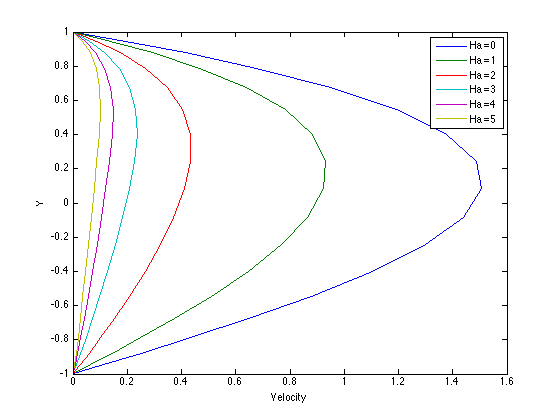
\includegraphics[scale=0.75]{figures/vel.png}
\end{center}
\caption{Velocity profile dependence to magnetic field.}
\label{velMagDep} 
\end{figure}

\begin{figure}
\begin{center}
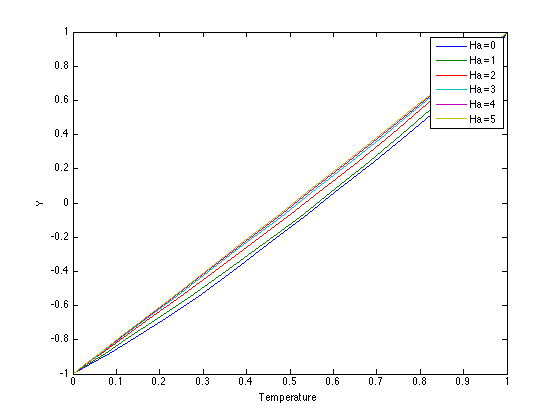
\includegraphics[scale=0.75]{figures/temp.png}
\end{center}
\caption{Temperature distribution dependence to magnetic field.}
\label{tempMagDep} 
\end{figure}


\section{Inclined Nanofluid Channel Flow}

In this section, the effect of parameters on thermal distribution and velocity profile are analyzed utilizing MATLAB. The particle volume fraction  $\psi $ is changed from 0 - 0.06, where $\psi  =0$ corresponding to the pure base fluid case without nanoparticles. Magnetic field effect on the flow is also investigated through changing the dimensionless $Ha$ number. The inclination angle dependence is briefly pointed. This part of the study is based on the work done in the author's paper \cite{baskaya2014investigation}.

Figure ~\ref{velMagDep} shows the effect of Hartmann number on the velocity profile.  Considered parameters for the simulation given in Fig ~\ref{velMagDep} and Fig ~\ref{tempMagDep} are $P = 1$; $Br = 0.1$; $Ra = 10$;  $Pr = 6.7$;  $\psi  =0.06$;  $\phi = pi/6$. As the Ha number increase the flow field is suppressed significantly due to the strong retarding effect of Lorentz force. This is also the case for fluids without nanoparticles but results show that for a concentration of $\psi  =0.06$, the magnetic field braking effect increases when compared to the case of no particles, i.e $\psi  =0$. Figure ~\ref{tempMagDep} also shows the temperature tendency vary almost linearly and decrease with increasing magnetic field intensity.


\begin{figure}
\begin{center}
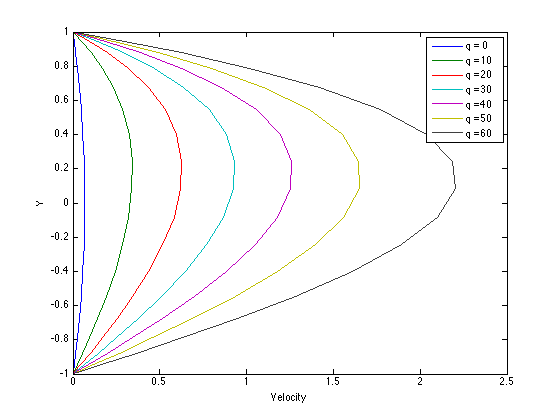
\includegraphics[scale=0.78]{figures/velocityIncAngDep.png}
\end{center}
\caption{Velocity profile dependence to inclination angle.}
\label{velincAngDep} 
\end{figure}

\begin{figure}
\begin{center}
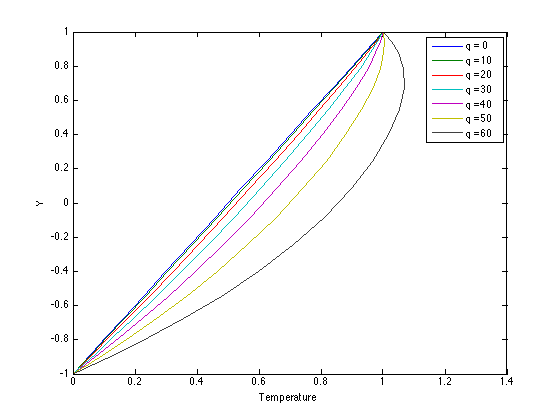
\includegraphics[scale=0.75]{figures/tempIncAngDep.png}
\end{center}
\caption{Temperature distribution dependence to inclination angle.}
\label{tempincAngDep} 
\end{figure}

\begin{figure}[t]
\begin{center}
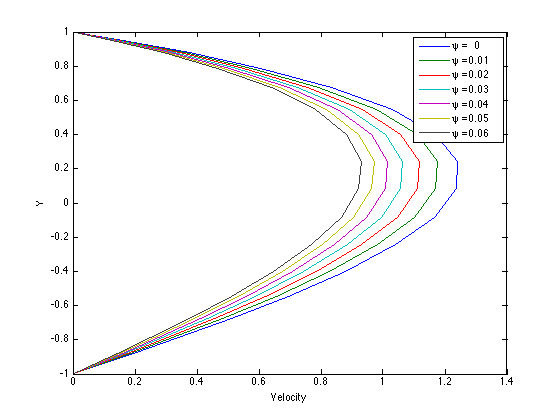
\includegraphics[scale=0.75]{figures/velConcentrationDep.png}
\end{center}
\caption{Velocity profile dependence to nanoparticle volume fraction.}
\label{velConcentrationDep} 
\end{figure}

\begin{figure}[t]
\begin{center}
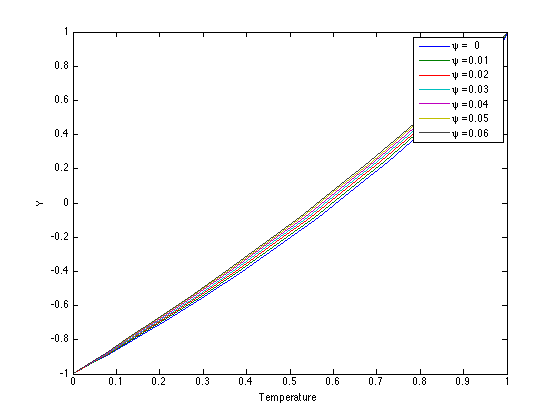
\includegraphics[scale=0.78]{figures/tempConcentrationDep.png}
\end{center}
\caption{Temperature distribution dependence to nanoparticle volume fraction.}
\label{tempConcentrationDep} 
\end{figure}



Figure ~\ref{velincAngDep} shows the velocity profile dependence on the inclination angle. Considered parameters for the simulation given in Fig ~\ref{velincAngDep} and Fig ~\ref{tempincAngDep} are $Ha = 1$;  $P = 1 $;  $Br = 0.1 $;  $Ra = 10 $;   $Pr = 6.7 $;  $\psi =0.06 $.The simulation converged for the inclination angle range $\phi = 0$ - $\phi = 60$ degrees but for larger angle values it diverged. The velocity dependence to inclination decreases with the addition of nanoparticles. The inclination dependence decreases  as magnetic field increases when there is no particles, i.e $\psi  = 0$. In nanofluid flow, the inclination dependence possess a similar tendency but not as strong as in clear water case.  Figure ~\ref{tempincAngDep} also shows that the temperature distribution is strongly dependent to inclination angle, temperature increases with increasing inclination angle. 

Figure ~\ref{velConcentrationDep} shows the velocity profile dependence on the volume fraction of nanofluids. Considered parameters for the simulation given in Fig ~\ref{velConcentrationDep} and Fig ~\ref{tempConcentrationDep} are $Ha = 1$; $P = 1$; $Br = 0.1$; $Ra = 10$; $Pr = 6.7$;  $\phi= pi / 6$. The velocity decreases with an increase in volume fraction of nanofluid. When magnetic field gets stronger, the volume fraction dependence of the velocity also increases and gets more dependent to temperature distribution.  The temperature distribution, given in Fig. ~\ref{tempConcentrationDep}, is not very effected by volume fraction and this dependence gets even less with increased magnetic field magnitude.

\section{Inclined Nanofluid Channel Flow Exposed to Oriented Magnetic Field}

In this section, simulations are carried out for a variety of parameters and solved via GDQM \&~NR methods. The velocity and temperature distributions, local entropy generation and total entropy generation are investigated with respect to key system parameters, such as magnetic field angle, inclination of the channel, Ha number and nanoparticle volume fraction.  The codes are implemented in MATLAB environment. This part of the study is based on the work done in the author's paper \cite{baskaya2017investigation}.


Since the numeric solution is designed in-house, the need to verify its validity, a simpler geometry is refered where numerical results are easily available in the literature and simplifies to an analytical solution under some conditions. This study adopts a suction-injuction channel flow without nanofluids. The results show that DQM tool implemented in-house gives even more accurate results then Runge-Kutta solutions given in  \cite{eegunjobi2013entropy} for the specific case where an analytical solution is also available for comparison \cite{bacskaya2014analysis}. Furthermore, another strong feature of DQM is observed, ability~to give relatively accurate solutions for few number of grids.
Further verification has been proceed with a comparison with the literature for trends of change of velocity and temperature profiles while parameters of the flow is changed such as Ha number.


This problem is designed such that the user of the system would have more parameters to configure the flow.
One of the main controllable parameter is angle of the magnetic field. Throughout this study, the direction of the magnetic field is not assumed to be perpendicular to the channel walls while the inclination of the channel is changing. This configuration might have been helpful to have an insight for the applications where inclination of the channel could not be changed but the magnetic field angle could be changed.  



\begin{figure}
\centerline{\psfig{figure=figures/tempDist.eps,width=5in}}
\vspace*{5mm}
\caption{Nondimensionalized temperature change with channel width for a variety of magnetic field intensity and solid volume fraction.}
\label{tempDist} 
\end{figure}


First of all, effect of magnetic field magnitude (discarding the direction) on the flow is investigated by changing the dimensionless $Ha$ number but keeping the magnetic field direction constant.  Considered parameters for the simulation given in Figures~\ref{tempDist} and~\ref{velDist} are $P = 1$; $Br = 0.1$; $Ra = 10$;  $Pr = 6.7$;  $\alpha  = 10\degree$;  $\phi = 30\degree$. Figures~\ref{tempDist} and~\ref{velDist} also shows the effect of nanoparticle volume fraction on velocity and temperature profiles. By letting more particles to the system or discarding some, the flow can be supervised. In the simulations, the particle volume fraction is changed between $\psi =$ 0--0.06  from  where $\psi  =0$ corresponding to the pure base fluid case without nanoparticles. The velocity decreases with an increase in volume fraction of nanofluid. %please confirm if it is correct

\begin{figure}
\centerline{\psfig{figure=figures/velDist.eps,width=5in}}
\vspace*{5mm}
\caption{Nondimensionalized velocity change with channel width for a variety of magnetic field intensity and solid volume fraction.}
\label{velDist} 
\end{figure}

 Figure~\ref{velDist} shows the effect of Hartmann number on the velocity profile. It is clear that, increasing the value of Ha have a tendency to slow down the fluid motion because of the presence of the transverse magnetic field. Transverse magnetic field creates a resistive force similar to the drag force, which acts in the opposite direction of the fluid motion. The velocity of the fluid decreases with resistive force and it is clear that the applied magnetic field has a retarding effect on the flow field. This is also the case for fluids without nanoparticles but results show that for a concentration of $\psi  =0.06$, the magnetic field braking effect increases when compared to the case of no particles, i.e., $\psi  =0$. 
 
 Figure~\ref{tempDist} shows the temperature variation is almost linear with respect to non-dimensionalized channel width and decrease with increasing magnetic field intensity. The fluid temperature decreases increasing the value of Ha within the channel due to increasing magnetic field intensity. This behavior is attributed to decrease the fluid velocity due to the magnetic field.


As mentioned above, the main parameter to be utilized in order to achieve more dominance over the behavior of the flow is the magnetic field angle $(\alpha)$. To further differentiate the effect of magnetic field and gravitation over the flow, the magnetic field angle is offered to be independent from the angle of the channel. This could be a good modeling approach for the problems where the channel has a~fixed inclination while the magnetic field can be directed independently. An example case could be an medical application where the veins should not be moved while the magnetic field applied from outside could be changed in favor of the application. 

\begin{figure}
\centerline{\psfig{figure=figures/velDistHa2vol006.eps,width=5in}}
\vspace*{5mm}
\caption{Nondimensionalized velocity with  respect to magnetic field angle $\alpha$ and  channel inclination~$\phi$.}
\label{velDistHa2vol006} 
\end{figure}



Figure~\ref{velDistHa2vol006} shows the behavior of the velocity along the channel for a variety of magnetic field and channel inclination values for $\psi = 0.06$ and $Ha = 2$. The rise in the inclination causing an increase in the flow velocity is observed, obviously matching the common sense. The velocity profiles are unsymmetrical about the centerline of the channel due to inclination angle as expected. It also shows that when the inclination of the magnetic field increased, the flow velocity decreases. A key point to realize is that the flow velocity can be decreased to a level less then even a higher inclination of the channel velocity profile by changing the magnetic field angle less then 45\degree. This can be seen clearly from the curves representing $\alpha = 0\degree,\, \phi = 10$ and $\alpha = 45\degree, \,\phi = 20\degree$ in Figure~\ref{velDistHa2vol006}. This gives the user of the channel a good dominance to control the flow as is intended. A second point in Figure~\ref{velDistHa2vol006} is that for higher values of magnetic field angle, the less change will be observed in the velocity change corresponding to a change in magnetic field angle. This can be observed by checking the same color curves, and realize that the difference of flow velocity suppression is higher in the change from $\alpha = 0\degree$ to $\alpha = 45\degree$ compared to the change in $\alpha = 45\degree$ to $\alpha = 90\degree$. The flow velocity supression in higher magnetic field inclinations also decreases for higher channel inclination. This can be seen by observing the decrease in velocity for $\alpha = 45\degree$ to $\alpha = 90\degree$ for $\phi = 20\degree$ is less than the decrease in velocity for $\alpha = 45\degree$ to $\alpha = 90\degree$ for $\phi = 10\degree$. Another result is that these behaviour does not change for different nano-particle volume fractions $\psi$ but not showed here due to page limitations. 


Figure~\ref{vel_3DHa2vol003} is a broader look at the trend of the effect of $\alpha$ and $\phi$ on flow velocity, by showing 3D figures representing the change of flow velocity with respect to inclination of the channel $\phi$ for four different magnetic field angle $\alpha$. The results discussed until now can be seen in this figure as well as a~trend in change in shape of the surface for different values of magnetic field angles $\alpha$.

\begin{figure}
\centerline{\psfig{figure=figures/vel_3DHa2vol003.eps,width=5in}}
\vspace*{6mm}
\caption{3D flow behaviour surface for nondimensionalized velocity with respect to channel inclination $\phi$ for four different magnetic field angle $\alpha$.}
\label{vel_3DHa2vol003} 
\end{figure}




Engineering system design is a complicated process and most of the times requires comprise from one property or another. A wise choice to tune in between favorable properties, there are various optimization methods. One of them is to calculate and minimize the entropy generation. 
The influences of the different parameters on entropy generation within the channel are presented in Figures \ref{localEntGenHa2vol006}--\ref{entGenModesHa2vol006}. It~is seen from Figures that the entropy generation depends on magnetic field angle, channel inclination.
Using~the local non-dimensional entropy generation rate formula for nanofluid in the presence of magnetic field is given in Equation (\ref{NS}), local entropy generation for a variety of $\alpha$~and $\phi$ for \mbox{$Ha =$ 2, }$\psi = 0.06$ and given in Figure \ref{localEntGenHa2vol006}. It shows that the entropy generation trend changes heavily for different channel inclination angle $\phi$. A change in magnetic field angle $\alpha$ may also effect the entropy generation abruptly. When the magnetic field angle is increased, a decrease in entropy generation is observed in Figure~\ref{localEntGenHa2vol006}. But this effect gets nearly negligible for higher values of magnetic field angle. This can be checked by investigating the distance in between the local entropy generation curves for $\alpha = 0\degree$--$45\degree$ and $\alpha = 45\degree$--$90\degree$. Furthermore, addition of nanoparticles decrease the local entropy generation but does not change the effect of $\alpha$ and $\phi$ on the local entropy generation. Here only the trend for $\psi = 0.06$ is given but  in the course of the study, the effect of $\alpha$ and $\phi$ on the local entropy generation is investigated for $\psi = 0, 0.03, 0.06$ but not all given due to the page constraints.  %please confirm if there have a comma         %please confirm if it is correct 

\begin{figure}
\centerline{\psfig{figure=figures/localEntGenHa2vol006.eps,width=5in}}
\vspace*{5mm}
\caption{Local entropy generation as a function of channel width for specific magnetic field angle $\alpha$ and  channel inclination $\phi$.}
\label{localEntGenHa2vol006} 
\end{figure}


\begin{figure}
\centerline{\psfig{figure=figures/localEntropy_3DHa2vol006.eps,width=4.7in}}
\vspace*{6mm}
\caption{Local entropy generation as a function of magnetic field angle and channel width for four different channel inclinations $\phi = 0\degree, 20\degree, 30\degree, 40\degree$.}
\label{localEntropy_3DHa2vol006} 
\end{figure}

\begin{figure}
\centerline{\psfig{figure=figures/totalEntGenHa2vol006.eps,width=4.7in}}
\vspace*{5mm}
\caption{Total entropy generation as a function of magnetic field angle $\alpha$ for a variety of channel inclination $\phi$.}
\label{totalEntGenHa2vol006} 
\end{figure}

The influences of the different parameters on entropy generation within the channel are presented in Figures \ref{localEntGenHa2vol006}--\ref{entGenModesHa2vol006}. It is seen from Figs that the entropy generation number NS depends on magnetic field angle, channel inclination.

To gain further insight about the behavior of local entropy generation as a function of magnetic field angle and channel inclination, four 3D graphes are presented as Figure~\ref{localEntropy_3DHa2vol006}. In this simulation $Ha = 2$ and $\psi = 0.06$. These four surfaces in Figure~\ref{localEntropy_3DHa2vol006} present the change of local entropy generation with magnetic field angle $\alpha$ for four different channel inclinations $\phi = 0\degree, 20\degree, 30\degree, 40\degree$.

\begin{figure}
\centerline{\psfig{figure=figures/entGenModesHa2vol006.eps,width=5in}}
\vspace*{5mm}
\caption{Total entropy generation due to its terms; heat transfer term, viscous dissipation term, magnetic field term as a function of magnetic field angle $\alpha$ for channel inclination $\phi = 20$.}   %it is different from picture, please confirm if it is italic
\label{entGenModesHa2vol006} 
\end{figure}

It can be seen from the upper left surface corresponding to $\phi = 0\degree$, the change in magnetic field angle $\alpha$ does not help much to decrease the local entropy generation. But for channel inclination $\phi = 20\degree$, local entropy generation is decreased for higher values of $\alpha$. For higher values of $\phi$, $\phi = 30\degree, 40\degree$, an increase in $\alpha$~first results in a decrease in local entropy generation. But after some specific value, the local entropy generation starts to increase for increasing $\alpha$. This can be seen also from Figure~\ref{totalEntGenHa2vol006}, where local entropy generation is averaged along the width of channel and no longer dependent on the location, namely~total entropy generation. Those result means that magnetic field angle can be used to decrease local entropy generation but depending on the inclination of the channel, this might be the contrary. This means that the user can utilize these behavior to optimize the system depending on the perquisites of the problem. Another result observed is that this behavior is not changed for nanoparticle volume fraction $\psi$. But for larger $\psi$, a general decreasing effect is seen in the simulations for all values of $\alpha$ and~$\phi$.
 

A further investigation given in Figure~\ref{entGenModesHa2vol006} on the total entropy generation concerns the visualization of entropy generation terms separately. As seen from Equation (\ref{equ26}), the entropy generations is comprised of entropy generation due to heat transfer irreversibility, entropy generation due to fluid friction irreversibility and  entropy generation due to magnetic field. Figure~\ref{entGenModesHa2vol006} shows that the decrease in total entropy generation via an increase in magnetic field angle belongs to viscous dissipation and magnetic field terms of entropy generation. The entropy generation term due to heat transfer irreversibility remains nearly unchanged. To achieve a further decrease in entropy generation, this~terms might be handled with a different controllable parameter. 
  


